\newpage
\section{2024年11月12日}
\begin{tcolorbox}[cyan]
    \begin{description}
        \item[\large \textbf{任务}]
        \item[1、] 读文献学习代价函数构建方法
        \item[2、] 解决优化轨迹“打圈”的问题
        \item[3、] 文献进展报告为四部分:(1)论文所解决的问题(2)算法(3)结果(4)论文启发 
    \end{description}
\end{tcolorbox}
\subsection{Minimum Snap Trajectory Generation and Control for Quadrotors(ICRA2011)}
\subsubsection{论文所解决的问题}
论文提出了四旋翼无人机在严格约束(轨迹总时间以及航点约束)的三维空间中的控制器设计和轨迹生成方法。
论文对无人机的微分平坦特性进行了详细推导;构建minimum snap优化问题,将优化变量的解耦关系,将问题分解成四个优化问题,并转换成无量纲优化问题。
并提出飞行走廊约束方法,本文中用于无人机钻环。
\subsubsection{论文算法}
(1)\textbf{无人机微分平坦特性}


无人机动力学模型如下:
\begin{subequations}
    \begin{numcases}{}
      m\ddot{\mathbf{r}}=-mg\mathbf{z}_W+u_1\mathbf{z}_B \label{dynamic1}\\
      \dot{\boldsymbol{\omega}}_{BW}=\mathcal{I}^{-1}\left[-\boldsymbol{\omega}_{BW}\times \mathcal{I}\boldsymbol{\omega}_{BW}+\left[\begin{array}{c}u_2\\u_3\\u_4\end{array}\right]\right]\label{dynamic2}
    \end{numcases}
\end{subequations}


平坦输出:$\sigma(t) = \left[x,y,z,\psi \right]^T $。由式\ref{dynamic1}可知,机体坐标系的$Z_B$轴方向$\mathbf{z_B}$满足下式
\begin{equation}\label{zBandt}
    \mathbf{z_B}=\frac{\mathbf{t}}{\left\lVert\mathbf{t} \right\rVert },\mathbf{t}= \left[\ddot{\sigma}_1,\ddot{\sigma}_2,\ddot{\sigma}_3 +g  \right]^T
\end{equation}
给定$\psi$,可以计算出$\mathbf{x}_C = \left[\cos\sigma_4,\sin\sigma_4,0  \right]^T$,由于采用$Z-X-Y$的旋转顺序,
坐标轴\(\mathbf{x}_C\)和\(\mathbf{x}_B\)、\(\mathbf{z}_B\)在一个平面,$\mathbf{y}_B$与$\mathbf{z}_B$和$\mathbf{x}_C$正交。
因此,有
\begin{equation}\label{flatness1}
    \mathbf{y}_B=\frac{\mathbf{z}_B\times\mathbf{x}_C}{\|\mathbf{z}_B\times\mathbf{x}_C\|},\begin{array}{c}\mathbf{x}_B=\mathbf{y}_B\times\mathbf{z}_B\end{array}
\end{equation}
之后可以唯一确定从机体坐标系到世界坐标系的旋转矩阵\(^WR_B=\left[\mathbf{x}_B\ \ \mathbf{y}_B\ \ \mathbf{z}_B\right]\),
通过旋转矩阵可以确定无人机的滚动角\(\phi \)和俯仰角$\theta$。对式\ref{dynamic1}求导得
\begin{equation}\label{equ-3-14}
    m\dot{\mathbf{a}}=\dot{u}_1\mathbf{z}_B+\boldsymbol{\omega}_{BW}\times u_1\mathbf{z}_B
\end{equation}
沿\(\mathbf{z}_B\)投影可得\(\dot{u}_1=\mathbf{z}_B\cdot m\dot{\mathbf{a}} \),
并定义向量\(\mathbf{h}_\omega=\boldsymbol{\omega}_{BW}\times\mathbf{z}_B=\frac m{u_1}(\dot{\mathbf{a}}-(\mathbf{z}_B\cdot\dot{\mathbf{a}})\mathbf{z}_B)\)
为\(\frac m{u_1}\dot{\mathbf{a}}\)在\(X_B-Y_B\)平面上的投影。因此
\begin{equation}
   p=-\mathbf{h}_\omega\cdot\mathbf{y}_B,q=\mathbf{h}_\omega\cdot\mathbf{x}_B\label{equ-3-15}
\end{equation}
另外,\(r\)是\(\boldsymbol{\omega}_{BW}\)在\(\mathbf{z}_B\)方向的分量,
并将\(\boldsymbol{\omega}_{BW}\)分解为\(\boldsymbol{\omega}_{BC}+\boldsymbol{\omega}_{CW}\)能够得出
\begin{equation}\label{equ-3-16}
    r=(\omega_{BC}+\omega_{CW})\cdot\mathbf{z}_B=\omega_{CW}\cdot\mathbf{z}_B=\dot{\psi}\mathbf{z}_W\cdot\mathbf{z}_B
\end{equation}
同样,对式\ref{dynamic1}求二阶导可以得出,角加速度也可以被平坦输出及其有限阶导数的函数表示。

对于控制输入\(u\),由式\ref{dynamic1}、\ref{zBandt}可知,净推力\(u_1=m\|\mathbf{t}\|\);
另外,由于角速度和角加速度是\(z\)及其导数的函数,因此可以通过式\ref{dynamic2}来计算输入\(u_2\),\(u_3\)和\(u_4\)。
综上,四旋翼无人机系统的12个状态和4个控制输入都可以写成平坦输出\(\sigma\)及其导数的形式。

(2)\textbf{轨迹生成}


轨迹表示为$m$段$n$阶多项式轨迹,如下
\begin{equation}
    \sigma_T(t)=\left\{\begin{array}{cc}\sum_{i=0}^n\sigma_{Ti1}t^i&t_0\leq t<t_1\\\sum_{i=0}^n\sigma_{Ti2}t^i&t_1\leq t<t_2\\\vdots\\\sum_{i=0}^n\sigma_{Tim}t^i&t_{m-1}\leq t\leq t_m\end{array}\right.
\end{equation}


优化问题的构建:
代价函数包含位置$\mathbf{r_T}$的$k_r$阶导的平方和偏航角$\psi$的$k_\psi$阶导的平方,如下
\begin{equation}
    \begin{aligned}\label{costfun}
        &\min&\int_{t_0}^{t_m}\mu_r\left|\left|\frac{d^{k_r}\mathbf{r_T}}{dt^{k_r}}\right|\right|^2+\mu_\psi\frac{d^{k_\psi}\cdot\psi_\mathbf{T}}{dt^{k_\psi}}^2dt&\\
        &\text{s.t.}&\sigma_T(t_i)=\sigma_i,&i=0,...,m\\
        & &\frac{d^px_T}{dt^p}|_{t=t_j}=0\text{ or free},&j=0,m; p=1,...,k_r\\
        & &\frac{d^py_T}{dt^p}|_{t=t_j}=0\text{ or free},&j=0,m; p=1,...,k_r\\
        & &\frac{d^pz_T}{dt^p}|_{t=t_j}=0\text{ or free},&j=0,m; p=1,...,k_r\\
        & &\frac{d^p\psi_T}{dt^p}|_{t=t_j}=0\text{ or free},&j=0,m; p=1,...,k_\psi
    \end{aligned}
\end{equation}
其中,$\mu_r$、$\mu_\psi$的作用是使积分量无量纲。由于$u_2,u_3$由位置的四阶导表示,并且$u_4$由偏航角的二阶导表示,因此取$k_r=4,k_\psi=2$
将优化变量$\sigma_{Tij}=[x_{Tij},y_{Tij},z_{T\boldsymbol{i}j},\psi_{Tij}]^T$
写成$4mn\times 1$的向量$\mathbf{c}$,则问题转换为一个QP问题,如下
\begin{equation}\label{qp}
    \begin{array}{cc}\min&c^THc+f^Tc\\\mathrm{s.t.}&Ac\leq b\end{array}
\end{equation}
(3)\textbf{无量纲优化}


式\ref{costfun}中的变量$x_T,y_T,z_T,\psi_T$是解耦的,因此可以将问题分离为四个优化问题。
考虑单一无量纲变量$\tilde{\omega}(\tau)$的优化问题,如式\ref{costfun1}所示。其中$\tau$代表无量纲时间。
\begin{equation}
    \begin{aligned}\label{costfun1}
    \text{min}&\quad\quad\int_0^1\frac{d^k\tilde{w}(\tau)}{d\tau^k}^2d\tau\\
    \text{s.t.}&\quad\quad\tilde{w}(\tau_i)=\tilde{w}_i,&i=0,...,m\\
    \quad&\frac{d^p\tilde{w}(\tau)}{d\tau^p}|_{\tau=\tau_j}=0\text{ or free},&\tau_j=0,1; p=1,...,k
\end{aligned}
\end{equation}
引入时间维度$t=\alpha \tau$和变量$\omega$,定义为$w(t)=w(\alpha\tau)=\beta_1+\beta_2\tilde{w}(\tau)$。
则问题\ref{costfun1}可变换为如下问题
\begin{equation}
\begin{aligned}\label{costfun2}
    &\text{min}&&\frac{\alpha^{2k-1}}{\beta_{2}}\int_{0}^{\alpha}\frac{d^{k}w(t)}{dt^{k}}dt&&\\
    &\text{s.t.}&&w(t_{i})=\beta_{1}+\beta_{2}\tilde{w}_{i},\quad i=1,...,m\\
    &&&\frac{d^{p}w(t)}{dt^{p}}|_{t=t_{j}}=0\mathrm{~or~free},\quad t_{j}=0,\alpha; p=1,...,k
\end{aligned}
\end{equation}
在问题\ref{costfun2}中边界条件在空间维度平移了$\beta_1$缩放了$\beta_2$,在时间维度缩放了$\alpha$。
因此,如果无量纲优化问题\ref{costfun1}的最优解是$\tilde{\omega}^*$,则问题\ref{costfun2}的最优解为
\begin{equation}
    w^*(t)=\beta_1+\beta_2\tilde{w}^*\left(t/\alpha\right)
\end{equation}
\textbf{整体优化思路}:对于问题\ref{costfun},在解耦后分别与问题\ref{costfun2}对应,得到时间放缩尺度$\alpha$与
和每个变量在空间中的变换$\beta_1,\beta_2$的比例关系。每个变量的时间放缩尺度相同,空间放缩尺度可以不同。


1)时间放缩
\begin{equation}
    \mathbf{r}_T^*(t)=\mathbf{\tilde{r}}_T^*(t/\alpha), \psi_T^*(t)=\tilde{\psi}_T^*(t/\alpha).
\end{equation}


2)空间放缩
\begin{equation}
    x_T^*(t)=x_0+(x_1-x_0)\tilde{x}_T^*(t/t_1),
\end{equation}
其中,$\tilde{x}_T^*(0)=0,\tilde{x}_T^*(1)=1$,且$\tilde{y}_T,\tilde{z}_T$也满足同样的关系。\\
(4)\textbf{飞行走廊}


定义$\mathbf{t}_i$为$\mathbf{r}_i$到$\mathbf{t}_{i+1}$的单位向量,则垂直距离向量定义为
\begin{equation}
    \mathbf{d}_i(t)=(\mathbf{r}_T(t)-\mathbf{r}_i)-((\mathbf{r}_T(t)-\mathbf{r}_i)\cdot\mathbf{t}_i)\mathbf{t}_i.
\end{equation}
并定义约束
\begin{equation}\|\mathbf{d}_i(t)\|_\infty\leq\delta_i\text{ while }t_i\leq t\leq t_{i+1}.\end{equation}
其中,$\left\lVert \right\rVert _\infty  $表示无穷范数。对于$n$维向量$\mathbf{x}=(x_{1},x_{2},\ldots,x_{n})$,无穷范数定义为$\|\mathbf{x}\|_\infty=\max_{1\leq i\leq n}|x_i|$。
上述约束可以通过引入$n_c$个中间点从而合并至QP问题\ref{qp}中。
\begin{equation}
    \left|\mathbf{x}_W\cdot\mathbf{d}_i\left(t_i+\frac{j}{1+n_c}(t_{i+1}-t_i)\right)\right|\leq\delta_i\text{ for }j=1,...,n_c
\end{equation}
(5)\textbf{时间优化}


在大多数情况下,飞至某个固定点时的时间并不重要,因此可以对这些时间进行优化,找到每段轨迹最优飞行时间。
构建如下优化问题。
\begin{equation}\label{optt}
    \begin{aligned}\min&f(\mathbf{T})\\\mathrm{s.t.}&\sum T_i=t_m\\&T_i\geq0\end{aligned}
\end{equation}
其中$f(\mathbf{T})$是问题\ref{costfun}的解,时间向量$\textbf{T}= [T_1,T_2,...,T_m]$。可通过梯度下降法来求解问题\ref{optt}。
$f(\mathbf{T})$对第$i$段轨迹的时间的导数如下
\begin{equation}
    \nabla_{g_i}f=\frac{f(\mathbf{T}+h\mathbf{g}_i)-f(\mathbf{T})}h
\end{equation}
其中,向量$\mathbf{g}_i$的第$i$个元素是1,其余元素都是$\frac{-1}{m-1}$。可以使得$\sum\mathbf{g}_i=0$,对轨迹飞行总时间没有影响。

\subsubsection{论文实验结果}
(1)飞行走廊、时间优化仿真实验
\begin{figure}[htbp]
    \centering
    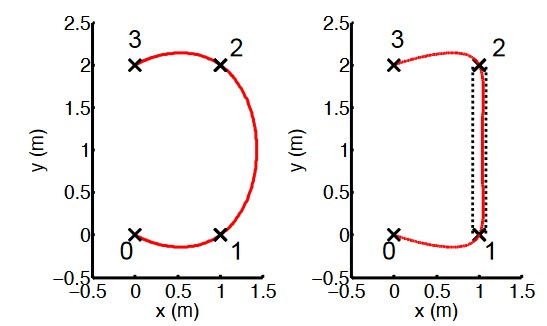
\includegraphics[width=8cm, height=4cm]{image/minimumSnap1.jpg}
    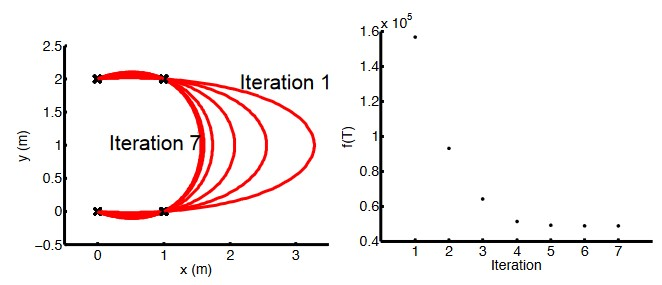
\includegraphics[width=8cm, height=4cm]{image/minimumSnap2.jpg}
    \caption{飞行走廊实验(左)  时间优化实验(右)}\label{snap1}
\end{figure}



(2)实机钻环实验
\begin{figure}[htbp]
    \centering
    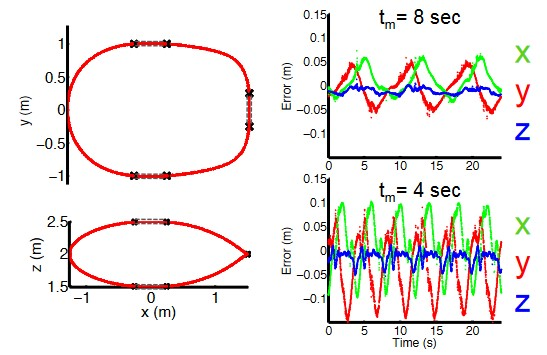
\includegraphics[width=8cm, height=5cm]{image/minimumSnap3.jpg}
    \caption{实机钻环实验}\label{snap3}
\end{figure}

\subsubsection{论文启发}
(1)微分平坦


掌握无人机微分平坦特性的推导,由平坦输出获得全状态变量和全输入变量的方法。


(2)优化问题各维度解耦与无量纲优化


在该优化问题中优化变量是解耦的,因此优化问题可以被分解为若干个优化子问题。
并且可以将子优化问题转换为无量纲优化问题,在得到无量纲优化问题的最优解后,
通过时空放缩即可得到原问题最优解。该方法比直接求解QP问题快速,对于快速响应动态障碍物或目标非常有效


(3)时间重分配


总时间固定的重分配方法。


(4)飞行走廊思想


通过约束垂直距离向量的无穷范数,定义一个长方体形飞行走廊,并通过对轨迹采样来满足该飞行走廊约束。
\subsubsection{Minimum Snap问题的一些思考}
(1)\textbf{为什么优化时每一段轨迹的时间需要已知?}


如果在目标函数$J(\textbf{T})$中,惩罚项只包括$vec,acc,jerk,snap$,那可以通过无限地增加时间来使得代价趋向于0,这种优化问题无意义。


(2)\textbf{轨迹多项式的阶次如何确定?}


对于最小化轨迹$s$阶导数问题,假设轨迹多项式阶次为$n$,有$m$段轨迹,轨迹维度$j$,参数量$mj(n+1)$,已知约束$(2s+m-1)j$。因此,则需满足
$n\geq \frac{2s-1}{m}$,因此多项式为$2s-1$阶次。
\subsection{Polynomial Trajectory Planning for Aggressive Quadrotor Flight in Dense Indoor Environments(ISRR2013)}
\subsubsection{论文所研究的问题}
论文在Minimum Snap工作的基础上,将Minimum Snap问题转化为无约束二次规划问题,并给出QP问题的闭式解。另外,对minimum snap和轨迹总时间进行权衡构建代价函数,
并展示了在该优化问题中时间权重不会影响轨迹形状的现象,根据此现象提出了一种先优化时间比例再对总轨迹时间进行放缩的优化思路。
\subsubsection{论文算法}
(1)\textbf{Minimum Snap问题}


定义两点之间多项式的惩罚函数为其$\mathbf{P}(t)$导数的平方。
\begin{equation}
    J(T)=\int_0^Tc_0P(t)^2+c_1P^{\prime}(t)^2+c_2P^{\prime\prime}(t)^2+\ldots+c_NP^{(N)}(t)^2dt=\mathbf{p}^TQ(T)\mathbf{p}
\end{equation}
其中,$\mathbf{p}$是多项式的系数向量。在本问题中,必须固定时间$T$去优化。因此,$M$个多项式段的代价为
\begin{equation}\label{fun1}
    J_{\text{total}} = 
    \begin{bmatrix}
    \mathbf{p}_1 \\
    \vdots \\
    \mathbf{p}_M
    \end{bmatrix}^T
    \begin{bmatrix}
    Q_1(T_1) \\
    & \ddots \\
    && Q_M(T_M)
    \end{bmatrix}
    \begin{bmatrix}
    \mathbf{p}_1 \\
    \vdots \\
    \mathbf{p}_M
    \end{bmatrix}^T    
\end{equation}


(2)\textbf{连续性约束}


对于一段多项式,可以采用式\ref{constraint1}来对多项式端点的导数进行约束。
\begin{equation}\label{constraint1}
    A_i\mathbf{p}_i=\mathbf{d}_i,\quad A_i=\begin{bmatrix}A_0\\A_T\end{bmatrix}_i,\quad\mathbf{d}_i=\begin{bmatrix}d_0\\d_T\end{bmatrix}_i
\end{equation}
对于相邻两段多项式,要满足第$i$段多项式的末端的导数和第$i+1$段多项式的末端的导数相等。
\begin{equation}
    A_{T,i}\mathbf{p}_i=A_{0,i+1}\mathbf{p}_{i+1}
\end{equation}
这些约束可以写成一组线性等式约束。
\begin{equation}\label{constraint2}
    A_{total}\begin{bmatrix}\mathbf{p}_1\\\vdots\\\mathbf{p}_M\end{bmatrix}=\begin{bmatrix}\mathbf{d}_1\\\vdots\\\mathbf{d}_M\end{bmatrix}
\end{equation}

(3)\textbf{无约束QP问题}


将连续性约束\ref{constraint2}带入目标函数\ref{fun1},如下
\begin{equation}
    J=\begin{bmatrix}\mathbf{d}_1\\\vdots\\\mathbf{d}_M\end{bmatrix}^T\begin{bmatrix}A_1\\&\ddots\\&&A_M\end{bmatrix}^{-T}\begin{bmatrix}Q_1\\&\ddots\\&&Q_M\end{bmatrix}\begin{bmatrix}A_1\\&\ddots\\&&A_M\end{bmatrix}^{-1}\begin{bmatrix}\mathbf{d}_1\\\vdots\\\mathbf{d}_M\end{bmatrix}
\end{equation}
其中,决策变量转化为多项式端点的导数。
对这些变量进行重新排序,将固定导数的变量$\mathbf{d_F}$分组在一起,自由导数的变量$\mathbf{d_F}$分组在一起,
这个变换由只有1和0组成的置换矩阵$\mathbf{C}$来完成。
如下
\begin{equation}
    J=\begin{bmatrix}\mathbf{d}_F\\\mathbf{d}_P\end{bmatrix}^T\underbrace{CA^{-T}QA^{-1}C^T}_R\begin{bmatrix}\mathbf{d}_F\\\mathbf{d}_P\end{bmatrix}=\begin{bmatrix}\mathbf{d}_F\\\mathbf{d}_P\end{bmatrix}^T\begin{bmatrix}R_{FF} R_{FP}\\R_{PF} R_{PP}\end{bmatrix}\begin{bmatrix}\mathbf{d}_F\\\mathbf{d}_P\end{bmatrix}
\end{equation}
\begin{equation}\label{qp1}
    J=\mathbf{d}_F^TR_{FF}\mathbf{d}_F+\mathbf{d}_F^TR_{FP}\mathbf{d}_P+\mathbf{d}_P^TR_{PF}\mathbf{d}_F+\mathbf{d}_P^TR_{PP}\mathbf{d}_P
\end{equation}
对$J$求微分并使其等于0,得到二次规划问题\ref{qp1}的闭式解
\begin{equation}
    \mathbf{d}_P^*=-R_{PP}^{-1}R_{FP}^T\mathbf{d}_F
\end{equation}


(4)\textbf{时间分配}


权衡Minimum Snap和总轨迹时间,构建如下代价函数
\begin{equation}\label{fun2}
    J_{\text{total}} = 
    \begin{bmatrix}
    \mathbf{p}_1 \\
    \vdots \\
    \mathbf{p}_M
    \end{bmatrix}^T
    \begin{bmatrix}
    Q_1(T_1) \\
    & \ddots \\
    && Q_M(T_M)
    \end{bmatrix}
    \begin{bmatrix}
    \mathbf{p}_1 \\
    \vdots \\
    \mathbf{p}_M
    \end{bmatrix}^T +k_T\sum_{i=1}^MT_i   
\end{equation}


采用梯度下降迭代求解,过程如下图所示
\begin{figure}[htbp]
    \centering
    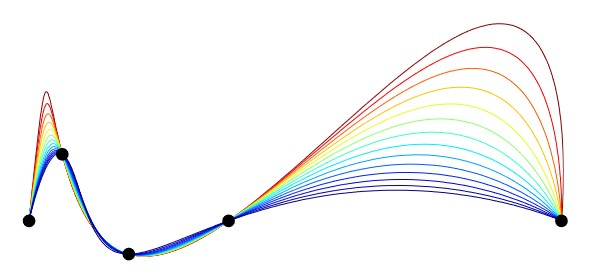
\includegraphics[width=8cm, height=4cm]{image/poly1.jpg}
    \caption{迭代过程,初始总时间为10.5s(红色),最优总时间为7s(蓝色)}\label{poly1}
\end{figure}


采用不同时间权重$k_T$进行优化,结果如下图所示
\begin{figure}[htbp]
    \centering
    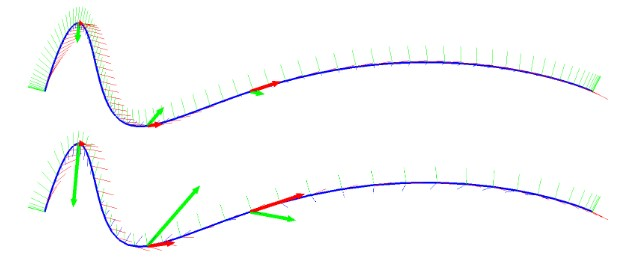
\includegraphics[width=8cm, height=4cm]{image/poly2.jpg}
    \caption{时间权重对比实验,$k_T$分别设置为 500(上)和 50000(下)}\label{poly2}
\end{figure}


最优轨迹时间分别为9.1s和5.1s,红色矢量为航路点速度、绿色为加速度。
论文提出无论$k_T$的值如何,最佳轨迹的几何形状都保持不变,最优轨迹段的时间比率与$k_T$无关。


(5)\textbf{轨迹避障}


论文采用的轨迹避障方法如下:
当优化后的轨迹与障碍物发生碰撞时,只需要在发生碰撞的轨迹段的两端之间插入一个额外的航路点,将该段路径分成两部分。
该航路点位于搜索算法给出的最佳分段路径上,因此是无碰撞的。插入新的航路点后重新优化多项式轨迹。并在碰撞时重复该过程。


(6)\textbf{执行器约束}


可行性的关键因素是确保轨迹在飞行过程中始终满足四旋翼飞行器的输入约束,基于四旋翼无人机的微分平坦特性,
可以将输入、动力学约束映射到平坦输出空间。

由于平坦输出空间中可行集的非凸性,可能并不能收敛到全局最优。因此,论文提出一种优化策略:
\begin{itemize}
    \item 首先忽略执行器约束,通过梯度下降优化分段时间比率。
    \item 利用最佳时间比率相对于总时间不变的现象,在达到最佳时间比率后,保留最佳比率对总轨迹时间进行优化。
\end{itemize}

\subsubsection{论文实验}
(1)\textbf{优化问题的解的质量}


    通过与采样方法(多项式RRT* )进行对比。
    \begin{figure}[htbp]
        \centering
        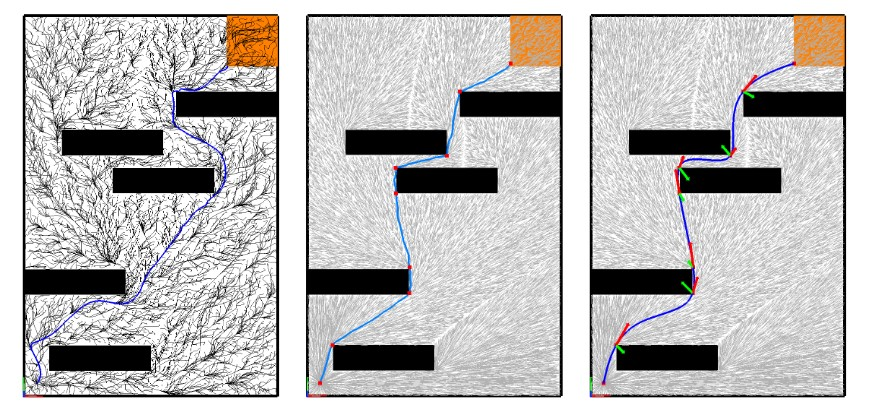
\includegraphics[width=12cm, height=5.5cm]{image/poly3.jpg}
        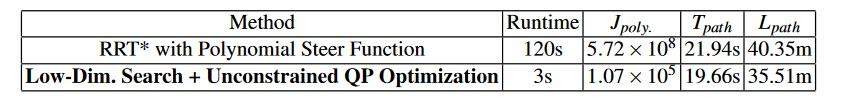
\includegraphics[width=12cm, height=1.5cm]{image/poly.jpg}
        \caption{多项式RRT*(左)、直线RRT*取航点进行优化(中)、优化(右)}\label{poly3}
    \end{figure}


(2)\textbf{优化性能}


    对比不同求解方法所用时间以及成功率,证明无约束优化算法的效率以及数值稳定性。
    \begin{figure}[htbp]
        \centering
        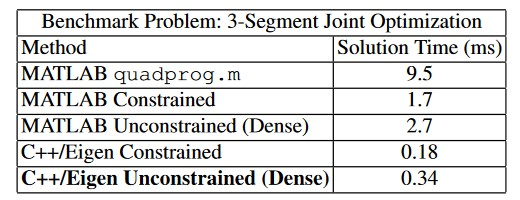
\includegraphics[width=8cm, height=3cm]{image/poly4.jpg}
        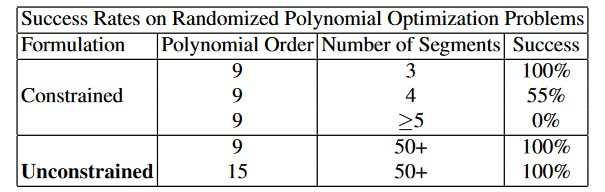
\includegraphics[width=8cm, height=3cm]{image/poly5.jpg}
        \caption{求解方法对比}\label{poly4}
    \end{figure}


(3)\textbf{实机实验}

\subsubsection{论文启发}
(1)Minimum Snap问题的闭式解。


(2)本文构建优化问题中,时间权重不影响最优轨迹形状。


(3)增加无碰撞的航路点来满足轨迹无碰撞。


(4)先优化时间比率,再考虑输入约束、动力学约束优化总轨迹时间的优化策略。